\documentclass[11pt]{article}
\usepackage{amsmath, amssymb, amsthm}
\usepackage[retainorgcmds]{IEEEtrantools}

\usepackage[pdftex]{graphicx}

\usepackage{marginnote}

\usepackage{fancyhdr}

%Format stuff
\pagestyle{fancy}
\headheight 35pt

%Header info
\chead{\Large \textbf{Derivatives}}
\lhead{}
\rhead{}

\begin{document}
\section{One Variable}
	\marginnote{Vector derivative properties?}If the derivative of a curve in space represented by $g(t)$ is continuous and never zero, then the curve is called \textbf{smooth}. Derivatives of vector equations work just as normal derivatives, except for a few new properties. In all examples, $\phi(t)$ and $u(t)$ are real, differentiable equations.
	\begin{IEEEeqnarray}{rCl}
		\frac{d}{dt}(\phi\vec{x}) & = & \phi\vec{x}' + \phi '\vec{x}\\
		\frac{d}{dt}(\vec{x}\cdot\vec{y}) & = & \vec{x}'\vec{y} + \vec{x}\cdot\vec{y}'\\
		\frac{d}{dt}(\vec{x}(u)) & = & u'(t)\vec{x}\prime(u)\\
		\frac{d}{dt}(\vec{x}\times\vec{y}) & = & \vec{x}'\times\vec{y} + \vec{x}\times\vec{y}'
	\end{IEEEeqnarray}
	
\section{Several Independent Variables}
	Thinking of functions as maps, a function in two variables (3D) is a map of $\mathbb{R}^2\rightarrow\mathbb{R}: (x,y,z) = (x, y, f(x,y))$. A four-dimensional graph would be a map of $\mathbb{R}^3\rightarrow\mathbb{R}$.
	
	\subsection{Level Sets}
		\marginnote{Level sets?}Even though 4D graphs are impossible to visualize, it is possible to visualize the graph at a given \textbf{level} $k$. The \textbf{level set} of $f$ at level $k$ is defined as follows:
		\begin{equation}
			L(k) = \{\vec{x}\}\in D(f) \mid f(\vec{x}) = k
		\end{equation}
		
	\subparagraph{Quadric Surfaces} Quadric surfaces \marginnote{Quadric surfaces?} are level sets in $\mathbb{R}^3$ of second-degree polynomials in 3 variables.
		
	\begin{figure}[htb]
		\centering
		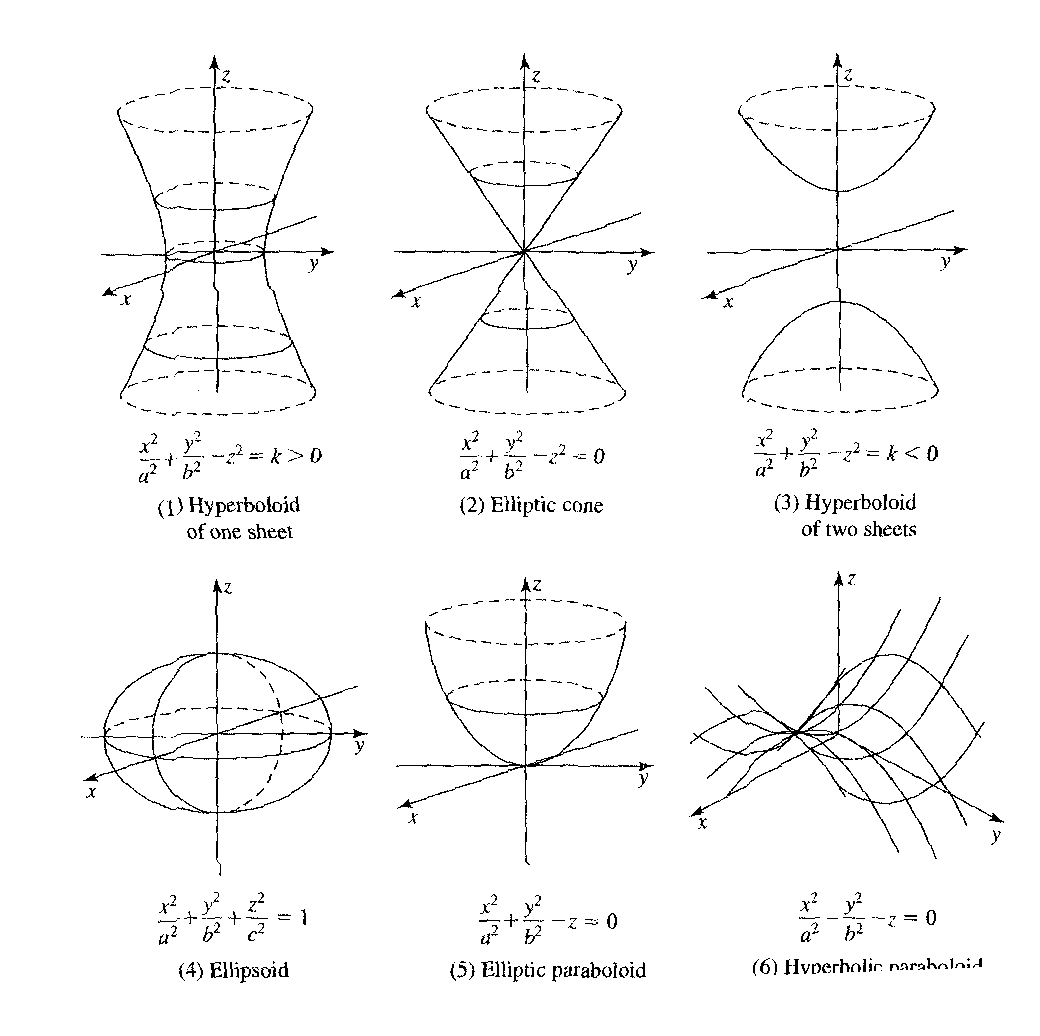
\includegraphics[width=0.8\textwidth]{quadric.png}
		\label{fig:quadric}
	\end{figure}
	
\section{Partial Derivatives}
	Taking a derivative of a function in two or more variables does not work in the traditional sense. Consider the definition of a derivative:
	\begin{equation}
		\frac{d}{dt}f(\vec{x}) = \lim_{\vec{h}\rightarrow\vec{0}} \frac{f(\vec{x}+\vec{h} - f(\vec{x)}}{\vec{h}}
	\end{equation}
	This expression cannot be evaluated because there is no definition of vector division or an inverse vector. To solve this problem, restrict $f$ to a parametric line.
	\begin{equation}
		\psi(t) = \vec{x}_0 + t\vec{v}, \vec{v} = \vec{e}_k
	\end{equation}
	
	\marginnote{Partials?}By reparametizing $f$ with $\psi$, we define the \textbf{partial derivative} of $f$ with respect to $x_i$ as follows.
	\begin{equation}
		\frac{\partial f}{\partial x_i} = \lim_{t\rightarrow 0}\frac{\vec{f}(\vec{x}_0 + t\vec{e}_i) - \vec{f}(x_0)}{t}
	\end{equation}
	
	This is equivalent to moving along a line in 1 dimension while keeping all dimensions constant. When computing a partial, derive with respect to the variable of the partial and treat all other variables as constants.
		
	\subsection{Geometric Interpretation}
		\subparagraph{Tangent Plane} The\marginnote{Geometry of partials?} function $f(x,y)$ can be restricted into a subset of $\mathbb{R}^2$ as $g(x) = f(x,b)$ and $h(y) = f(a,y)$. Then $\dfrac{\partial f}{\partial x}(a,b) = g'(a)$ and $\dfrac{\partial f}{\partial y}(a,b) = h'(b)$, where $g'(a)$ and $h'(b)$ describe the lines tangent to the two curves contained in $f$. 
		
		\marginnote{Tangent plane?}From the description of a plane:
		\begin{IEEEeqnarray}{rCl}
			z & = & \hat{\mathbf{n}} \cdot(\vec{x}-\vec{x}_0)\\
			z & = & \left(\frac{\partial \vec{f}}{\partial x} \times \frac{\partial \vec{f}}{\partial y}\right) \cdot (\vec{x} - \vec{x}_0)\\
			z & = & f(\vec{x}_0) + (x-a)f_x (\vec{x_0}) + (y-b)f_y (\vec{x_0})
		\end{IEEEeqnarray}
		
		\subparagraph{Clairaut's Theorem} Let $\mathbb{R}^2 \xrightarrow{f} \mathbb{R}$ be continuous ($\lim_{\vec{z}\rightarrow\vec{x}} f(\vec{z}) = f(\vec{x})$) and such that $f_x, f_y, f_{xy}, f_{yx}$ are also continuous on the same domain. Then $f_{xy} = f_{yx}$
		
\section{Parametrized Surfaces}
	When all coordinates but one in a vector are held fixed and the remaining $x_i$ is allowed to vary, then $f(\vec{x}): \mathbb{R}^n\rightarrow \mathbb{R}^m$ traces a \textbf{coordinate curve} in $\mathbb{R}^m$ given that $m\geq n$. The partial $\dfrac{\partial f}{\partial x_i}(\vec{x})$ is a tangent vector to the curve at the point $f(\vec{x})$.
	
	\subparagraph{Tangent Planes} The tangent plane to a surface $f(u, v)$ is described as $\vec{x} = s\vec{f}_u(u_0, v_0) + t\vec{f}_u(u_0, v_0) + \vec{f}(u_0,v_0)$.
	
	\subparagraph{Smoothness} A surface $S: \mathbb{R}^2\xrightarrow{g} \mathbb{R}^3$ is smooth at points $g(u,v)$ if there is a rectangle containing $(u,v)$ such that $g_u$ and $g_v$ are continuous and linearly independent. Intuitively, this means that the tangent plane is always varying at $g(u,v)$. A point where a surface is not smooth is called a \textbf{singular point}.
	
\section*{Important Concepts}
	\begin{itemize}
		\item The (partial) derivative of a vector is the same as deriving each component separately then combining.
		\item A level set at $k$  is $f(\mathbb{R}^n) = k \mid n\geq 3$.
		\item Equation of tangent plane comes from the cross product of two tangent vectors at the same point of a curve in space.
	\end{itemize}
%	\begin{center}
%	\begin{tikzpicture}
%		[scale=3,line cap=round,
%		%Styles
%		axes/.style=,
%		important line/.style={very thick},
%		information text/.style={rounded corners,fill=red!10,inner sep=1ex},
%		dot/.style={circle,inner sep=1pt,fill,label={#1},name=#1}			
%		]
%		
%		%Colors
%		\colorlet{anglecolor}{green!50!black}	%angle arcs/lines
%		
%		%The graphic
%	\end{tikzpicture}
%	\end{center}

%	\begin{figure}[htb]
%		\centering
%		\includegraphics[width=0.8\textwidth]{filename.eps}
%		\caption{Caption.}
%		\label{fig:figure}
%	\end{figure}

%		\def\enotesize{\normalsize}
%		\theendnotes
\end{document}